% \addcontentsline{toc}{chapter}{Chapitre 2} 
\chapter{Conduite du projet}

Ce chapitre est consacré à la conduite du projet. Il présente la méthodologie adoptée pour la conduite du projet ainsi que son plan et les outils utilisés pour faire la gestion de ce projet.

\clearpage
\label{sec:organisme}

\section{Introduction}
Dans le cadre de la conduite du projet d'ajout de nouvelles fonctionnalités dans l'application SG CONNECT, notre équipe, Bank UP, suit la méthodologie SCRUM. Notre priorité absolue est de satisfaire le client en fournissant rapidement des fonctionnalités à valeur ajoutée, en tirant parti du changement comme une opportunité. Dans ce chapitre, nous détaillerons les composants et les démarches de SCRUM que nous utilisons pour mener à bien ce projet, de la planification à la livraison finale. Notre approche SCRUM nous permet d'offrir des résultats de haute qualité dans des délais raisonnables, en favorisant la flexibilité et l'adaptation continue aux besoins changeants du projet.

\section{Méthodologie de travail : SCRUM}
La conduite de ce projet s'appuie sur la méthodologie SCRUM, adoptée par l'équipe de la Digital Factory pour garantir des résultats rapides et un time to market réduit. SCRUM est une approche agile qui permet une meilleure organisation des différentes phases du projet, en accordant une importance primordiale à l'implication et à la participation active du client tout au long du processus de développement. En suivant SCRUM, nous visons à améliorer la productivité de notre équipe, à respecter les délais fixés et à assurer le bon déroulement général du projet.

\begin{figure}[!h]
    \centering %
        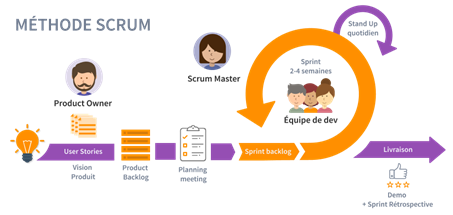
\includegraphics[width=14cm]{images/conduite/SCRUM.png}
    \caption{Méthode SCRUM}
\end{figure}

\textbf{\large{Les avantages de la méthode SCRUM}}
\medskip
\begin{itemize}
    \item[•] \textbf{Personnel engagé :} SCRUM favorise l'engagement du personnel en les impliquant activement dans la définition des activités et des horaires, ce qui conduit à une plus grande motivation et implication.
    \item[•] \textbf{Meilleure vue d’ensemble du projet :} SCRUM permet à tous les membres de l'équipe d'avoir une compréhension homogène des objectifs et des tâches à accomplir, offrant ainsi une meilleure vue d'ensemble du projet.
    \item[•] \textbf{Mise à jour des priorités :} Avec SCRUM, le client bénéficie d'une flexibilité au niveau de la définition et de l'évolution des priorités et des séquences d'activités, permettant une adaptation aux besoins changeants.
    \item[•] \textbf{Qualité du produit mise en avant :} SCRUM se concentre davantage sur la fourniture d'un service de valeur au client plutôt que sur une date limite stricte, mettant ainsi en avant la qualité du produit.
    \item[•] \textbf{Communication renforcée :} SCRUM favorise une communication régulière et transparente au sein de l'équipe, permettant une collaboration efficace et une résolution rapide des problèmes.
    \item[•] \textbf{Réduction des risques :} En utilisant des itérations courtes et des revues régulières, SCRUM permet de détecter et de résoudre les problèmes plus rapidement, réduisant ainsi les risques liés au projet.\\
\end{itemize}


\textbf{\large{Répartition des rôles dans SCRUM}}
\medskip
\begin{itemize}
    \item[•] \textbf{Le Scrum Master :} Il est responsable de la compréhension, de l'adhésion et de la mise en œuvre de la méthode SCRUM. Le Scrum Master facilite la communication au sein de l'équipe et cherche à maximiser sa productivité. Il veille également au respect des principes et des valeurs de SCRUM.
    \item[•] \textbf{Le Product Owner :} Il porte la vision du produit à réaliser et travaille en interaction avec l'équipe de développement. Le Product Owner établit les priorités des fonctionnalités à développer ou à corriger et valide les fonctionnalités terminées. Il est responsable de la gestion du product backlog et s'assure que les besoins du client sont correctement pris en compte.
    \item[•] \textbf{L'équipe de développement :} Elle est chargée de transformer les besoins définis par le Product Owner en fonctionnalités utilisables. Les décisions au sein de l'équipe de développement sont prises collectivement, sans notion de hiérarchie.\\
\end{itemize}


\textbf{\large{Les différents événements de la SCRUM}}
\medskip
\begin{itemize}
    \item[•] \textbf{Le sprint :} Il s'agit d'une itération de quelques semaines pendant laquelle une version terminée et utilisable du produit est réalisée. Un nouveau sprint commence immédiatement après la fin du précédent. Chaque sprint a un objectif clair et une liste de fonctionnalités à réaliser.
    \item[•] \textbf{La planification d'un sprint :} C'est une réunion qui précède le début d'un sprint et qui vise à définir les tâches à accomplir pendant cette période. L'équipe de développement et le Product Owner collaborent pour déterminer les objectifs et les priorités du sprint.
    \item[•] \textbf{La revue de sprint :} À la fin de chaque sprint, une réunion de revue est organisée pour présenter les fonctionnalités réalisées à l'équipe de développement et aux parties prenantes. C'est l'occasion de valider ce qui a été accompli et de recueillir des feedbacks.
    \item[•] \textbf{La rétrospective de sprint :} Elle se tient après la revue de sprint et permet à l'équipe de passer en revue le sprint écoulé afin d'identifier les aspects positifs, les problèmes rencontrés et les opportunités d'amélioration. Cela permet d'ajuster les pratiques et d'optimiser la performance pour les sprints suivants.
    \item[•] \textbf{Le daily scrum :} C'est une réunion quotidienne de courte durée au cours de laquelle l'équipe de développement fait le point sur sa progression. Les membres de l'équipe répondent à trois questions clés : qu'ont-ils réalisé la veille, qu'accompliront-ils aujourd'hui et quels sont les obstacles éventuels.\\
\end{itemize}

\textbf{\large{Les artefacts de SCRUM}}
\medskip
\begin{itemize}
    \item[•] \textbf{Le product backlog :} Il s'agit d'une liste hiérarchisée des exigences initiales du client concernant le produit à réaliser. Ce document évolue tout au long du projet en fonction des besoins du client, et le Product Owner en est responsable.
    \item[•] \textbf{Le sprint backlog :} Il représente le plan détaillé de la réalisation des objectifs d'un sprint, regroupant l'ensemble des user stories que l'équipe s'est engagée à accomplir. Il est défini lors de la réunion de planification du sprint et est régulièrement mis à jour pour suivre la progression.
    \item[•] \textbf{L'incrément :} Il correspond à la somme des éléments terminés du product backlog au cours d'un sprint, ainsi que des incréments des sprints précédents. À la fin d'un sprint, l'incrément doit être "Done", c'est-à-dire utilisable et conforme à la définition de "Done" définie par l'équipe SCRUM. Le Product Owner décide de sa libération ou non.
\end{itemize}


\section{Cycle de vie du projet}

\par Afin d’assurer le bon déroulement du projet, nous avons opté pour le cycle de vie suivant :
\begin{itemize}
    \item[$\bullet$] \textbf{Etude de cadrage:} cette étape consiste à bien définir le périmètre fonctionnel du projet. Elle permet de comprendre et analyser la structure de l’existant pour bien cadrer les besoins du client afin d’aboutir à un résultat qui s’aligne parfaitement avec ses attentes.
    \item[$\bullet$] \textbf{Spécifications et analyse des besoins:} cette phase permet de spécifier les besoins
définis dans la précédente phase du projet. Elle est d’une grande signification, 
    \item[$\bullet$] \textbf{Développement:} C'est la partie où l'on développe les fonctionnalités et les besoins exprimés lors de la phase précédente. L'objectif est de produire des services conformes aux spécifications exprimées par le métier tout en respectant un ensemble de règles de gestion technique et de bonnes pratiques.
    \item[$\bullet$] \textbf{Tests et validation:} Ils sont réalisés à la fin de chaque Sprint pour valider le travail réalisé avec le client.
    \item[$\bullet$] \textbf{Déploiement:} C'est la partie où les services développés et testés sont déployés dans un environnement accessible au client pour qu'il puisse les utiliser.
    \item[$\bullet$] \textbf{Monitoring:} À ce niveau, nous gardons un œil sur l'application en cours d'exécution et sommes prêts pour résoudre tout problème lorsqu'il se produit. 
\end{itemize}


\section{Planification du projet}
Pour gérer le projet et aboutir aux objectifs fixés ci-dessus, nous avons suivi les étapes représentées dans le diagramme de GANTT suivant :

\begin{figure}[!h]
    \centering %
        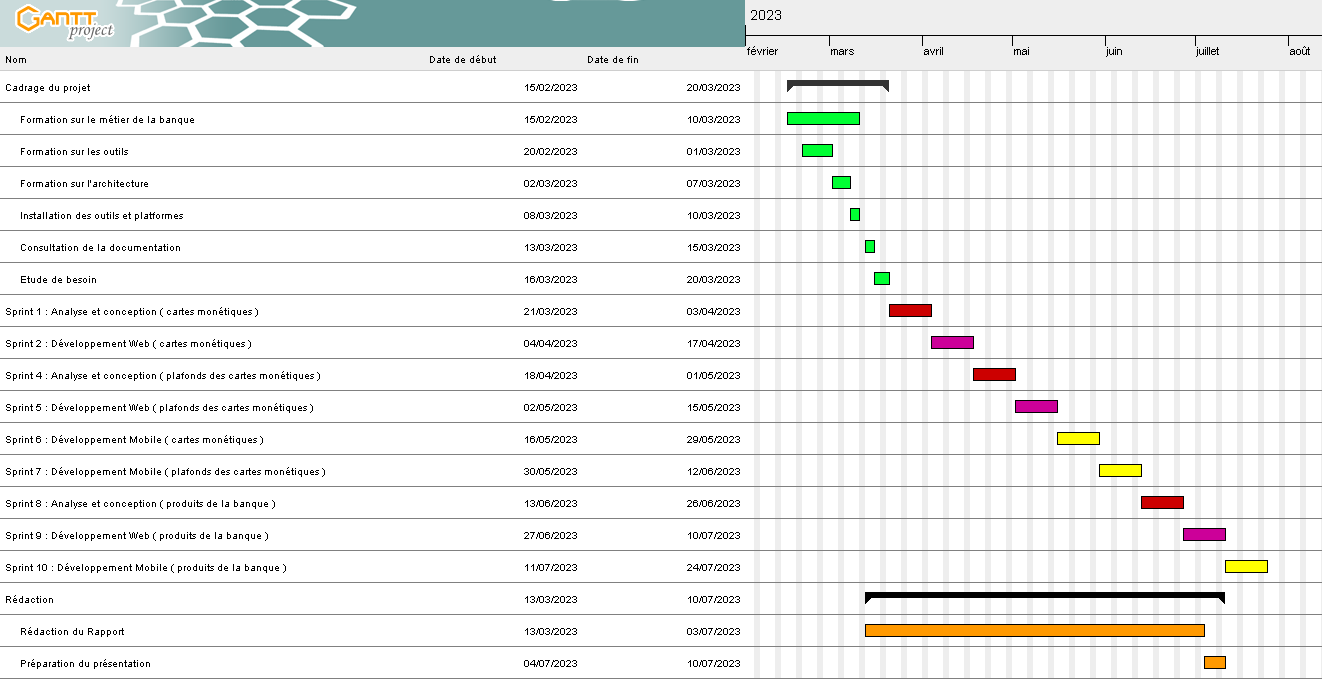
\includegraphics[width=16cm]{images/conduite/gantt.png}
    \caption{Diagramme de Gantt}
\end{figure}

\newpage

La phase de planification du projet a débuté par une étape de cadrage, au cours de laquelle nous avons bénéficié de formations approfondies afin de comprendre le domaine bancaire et de nous familiariser avec les exigences spécifiques du projet. Cette phase nous a permis de mener une étude approfondie des besoins et de spécifier les fonctionnalités à mettre en œuvre.\\

Pour mettre en pratique la méthodologie SCRUM, nous avons créé un backlog qui regroupe toutes les fonctionnalités requises sous forme de user stories. Lors de la réunion de planification du sprint, appelée "sprint planning", nous avons sélectionné les user stories sur lesquelles nous allons travailler pour chaque sprint. Ensuite, nous avons procédé à l'analyse et à la conception de chaque fonctionnalité, avant de passer à sa mise en œuvre.\\

Le développement de chaque fonctionnalité s'est déroulé au sein de sprints définis, où elle a été développée, testée, corrigée et déployée. À la fin de chaque sprint, nous avons obtenu une version fonctionnelle du produit, prête à être évaluée et validée par l'équipe de développement et les parties prenantes.\\

Cette approche itérative nous a permis de travailler de manière efficace et d'assurer une progression continue du projet, tout en offrant une flexibilité pour s'adapter aux éventuels changements de priorités ou de besoins.


\section{Outils de gestion de projet}

Pour mener à bien le projet, l'utilisation d'outils de gestion est essentielle afin de faciliter le travail d'équipe et de garantir le respect de la méthodologie Scrum. Trois outils ont été employés dans ce contexte : Jira, Microsoft Teams et Confluence.

\begin{itemize}
\item[$\bullet$] \textbf{Jira}
\end{itemize}
Jira a été utilisé comme outil de gestion de projet en ligne par la Société Générale African Business Services. Il s'agit d'une plateforme polyvalente qui facilite la gestion de projet en permettant le suivi des tâches, l'identification des obstacles et le partage d'informations au sein de l'équipe. Jira est basé sur l'organisation des projets en tickets, chacun représentant une tâche spécifique. Il offre également la possibilité de suivre l'état des tickets et de définir un flux de travail adapté aux méthodes de travail.\\
Jira génère des graphiques et des visualisations qui permettent de visualiser rapidement l'état des différentes missions et d'identifier les problèmes à résoudre en priorité.\\
Dans notre projet, Jira a été utilisé pour publier les User Stories, organiser les sprints et le backlog, suivre les tâches et sous-tâches, ainsi que pour estimer l'effort de l'équipe.
\begin{figure}[!h]
    \centering %
        
\includegraphics[height=3cm]{images/logos/jira.png}
    \caption{Logo de Jira}
\end{figure}

\begin{itemize}
    \item[$\bullet$] \textbf{Microsoft Teams}
    \end{itemize}
    Microsoft Teams a été utilisé pour organiser les réunions entre les membres de l'équipe. Cet outil a permis aux membres de l'équipe de communiquer, de planifier les tâches, de partager des astuces utiles, de discuter des progrès réalisés, des tâches à accomplir et des difficultés rencontrées. Des sessions de formation ont également été programmées pour renforcer la compréhension des fondements du métier bancaire dans notre domaine. Microsoft Teams a également été utilisé pour planifier les différentes cérémonies Scrum.
    \begin{figure}[!h]
        \centering %
            
\includegraphics[height=3cm]{images/logos/microsoftTeams.png}
        \caption{Logo de Microsoft Teams}
    \end{figure}

    \begin{itemize}
        \item[$\bullet$] \textbf{Confluence}
        \end{itemize}
        Confluence est une solution de travail collaboratif qui permet de créer et de stocker des fichiers sur une plateforme unique. Il offre la possibilité de créer des pages à partir de zéro ou d'utiliser des modèles personnalisables parmi une large sélection. Les pages créées peuvent être enrichies en commentaires, images, vidéos ou GIF, et peuvent être liées dans un espace dédié, permettant aux membres de l'équipe de partager leurs impressions, de demander de l'aide et de faciliter la prise de décision.
        \begin{figure}[!h]
            \centering %
                
\includegraphics[height=3cm]{images/logos/Confluence.png}
            \caption{Logo de Confluence}
        \end{figure}

Ces trois outils ont joué un rôle essentiel dans la gestion du projet en favorisant la collaboration, l'organisation et le partage d'informations au sein de l'équipe de développement.

\newpage

\section{Conclusion}
En conclusion de ce chapitre sur la conduite de projet, nous avons présenté la méthodologie adoptée, le cycle de vie du projet et la planification à l'aide du diagramme de Gantt. Nous avons également examiné les outils de gestion du projet utilisés pour faciliter la coordination et le suivi de l'équipe. Ces éléments sont essentiels pour assurer une gestion efficace du projet, respecter les délais et atteindre les objectifs fixés.\\
Dans le chapitre suivant, nous aborderons l'analyse des besoins, la modélisation et la conception du projet.